Experiment five was conducted because we saw that the system performance was directly related to number of hours (unseen data) it had to predict and where the offset for the prediction was set.
\subsection{Step-ahead forecasting}
\label{sec:stepAheadDiscussion}
The step-ahead experiments shows how each step are based on the step before it; because we include the last-known price (in the price predictions) and the last-known wind production(in the wind production predictions). When steps increase then the accuracy will decline thus introducing larger errors. This is because there is a certain elevation of error in our predictions because of the aforementioned last-known price and last-known wind production. In both of our results we see an improvement in the MAE with fewer hours to predict ahead. We also see that the elevation of the error at some point flattens thus not rising uncontrollably. This is because the other input parameters also influences the prediction (and not only the last-known price/wind production) thus guiding the prediction in the right direction. The step-ahead forecasts shows how important it is to use the predicted values and simulate a real life setting when doing the benchmarks for the specific dataset. If we did not use the predicted price when doing the next prediction in a 24 step-ahead forecast and if we instead used the exact value; then we would just be doing a 1 step-ahead forecast (as in figure \ref{fig:1HourAheadPrice_Discussion}) in 24 hour chunks. This again cements the need for transparency in what is done during a simulation to be able to reproduce the experiment but also be able to verify the results.

\begin{figure}[H]
\centering
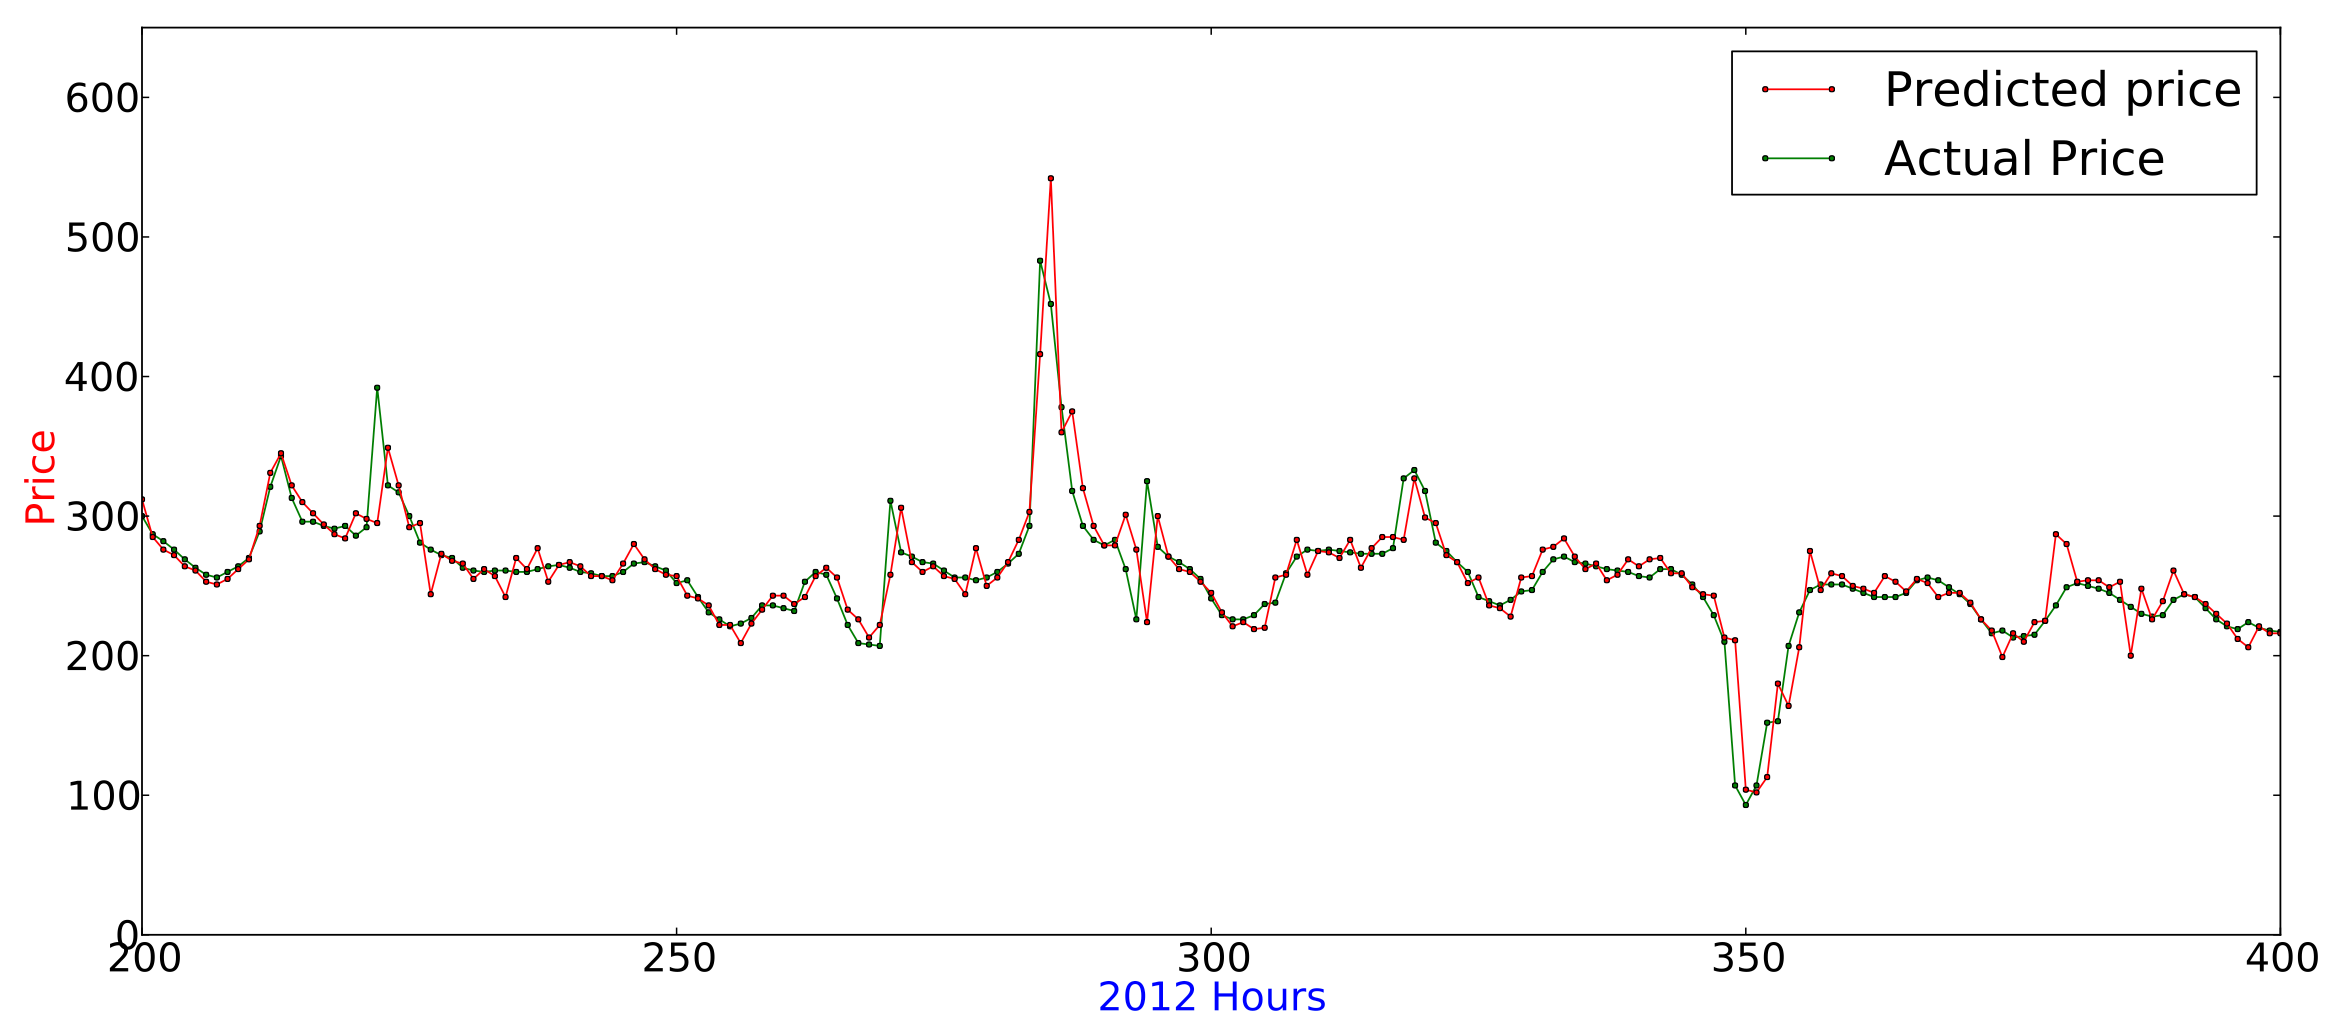
\includegraphics[width=0.99\linewidth]{billeder/Discussion/1HourAhead_Price.png}
\caption{The electricity price 1 hour-ahead forecast}
\label{fig:1HourAheadPrice_Discussion}
\end{figure}

This is a place where we can improve our algorithms since the error margin introduced by x hours-ahead are significant. Future work in this area includes predicting the next hour several times and taking the average of this thus reducing the error of one faulty prediction. This should help the ANN to limit the elevation of the error. Another approach would be to include the predicted step into the dataset and train the network again including the newest prediction thus adjusting the weights to accommodate the most recent prediction. The future work also includes looking into ways of eliminating the last-known price as an input thus eliminating the source of the elevation in errors. This could include a scatter scheme similar to the one presented in \cite{singhal2011electricity}. The step-ahead predictions also verifies the need for the predictions to be done on unseen data (as described in Section \ref{sec:inputParameterDiscussion}) and the need for simulation of unknown prices during the 24 hours we want to predict. 

\begin{figure}[H]
\centering
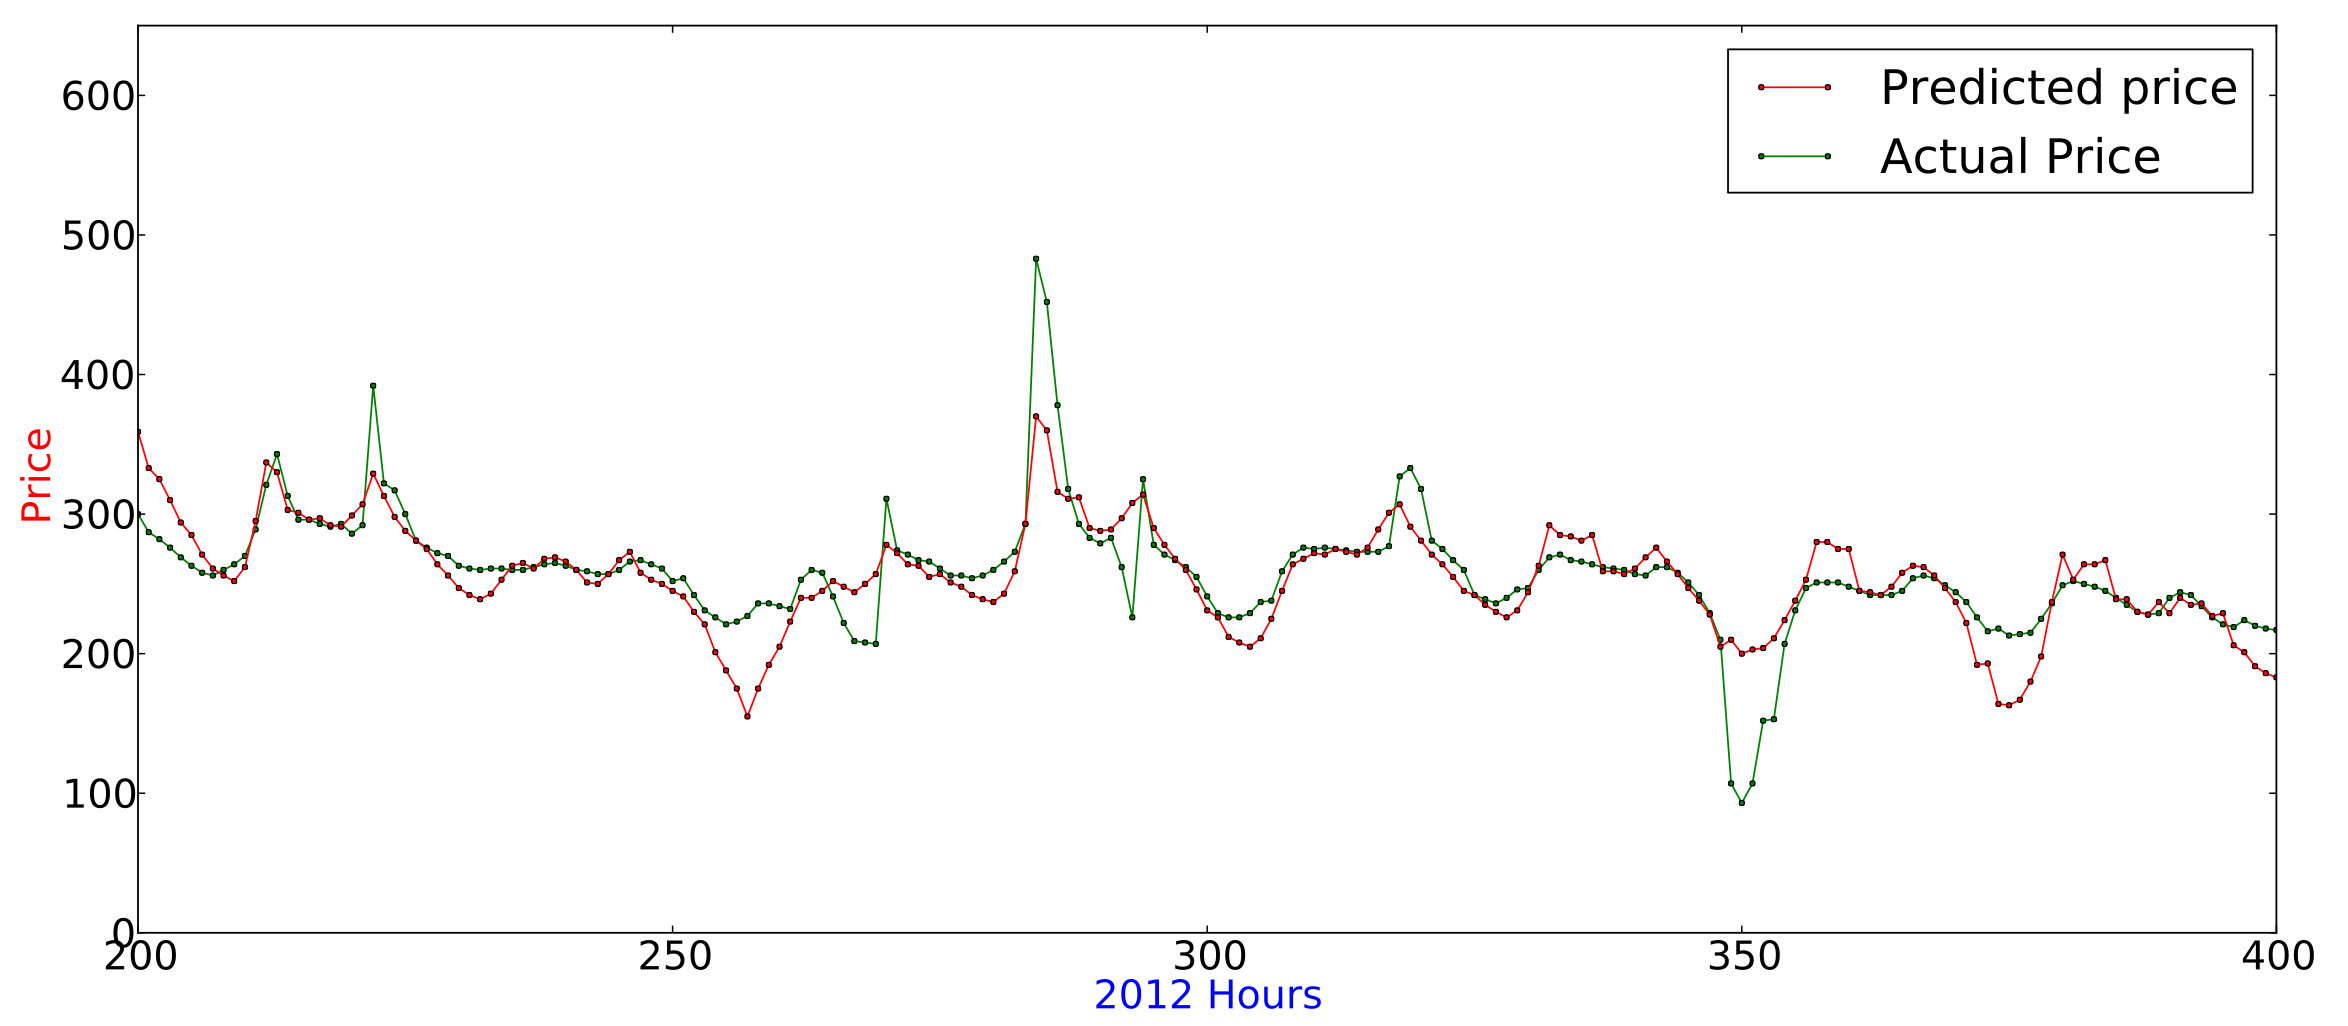
\includegraphics[width=0.99\linewidth]{billeder/Discussion/24HourAhead_Price.png}
\caption{The electricity price 24 hours-ahead forecast}
\label{fig:24HourAheadPrice_Discussion}
\end{figure}

\subsection{Offsets}
\label{sec:offsetsDiscussion}
Another source of errors are the changing offsets in the predictions. When we (in the previous experiment) change the number of hours to be predicted ahead we also change the offsets used to predict from. Some of the offsets in the dataset are better starting points (for a prediction) than others - reflected in the Table \ref{table:stepAheadForecastingWindProductionStartingPositions} and in Table \ref{table:Offsets} with an improvement of 23,34\% and 15,04\% respectively. The offsets in the dataset are not something that is covered in other papers (that we have read) which demonstrates the need for an expressive data analysis/experiment section that clarifies what they know about the dataset and how the predictions are affected. We also see papers that only use 1-2 weeks\cite{yamin2004adaptive} or only days \cite{1, singhal2011electricity, pjmForecast} for their test datasets. These papers do not state anything about changing offsets or what time of day they begin the prediction. When they have relatively small testing datasets the error from the right offsets will be significant thus we see a need for addressing it. Jonsson et al.\cite{forecastingSpotPricesAccountingForWindPower} writes that they do predictions from midnight to midnight to resemble how day-ahead forecasts are done in practice. This point is valid but still does not account for the offset problem. As we discussed in Section \ref{sec:unseenDataDiscussion} the need for testing all the different possibilities are important to get a full picture of how well a solution predicts the prices. If a setup was to be used in a live setting the changing offsets should be considered when stating how well a system performs. Also if this is not stated clearly in papers we can only make assumptions about how they subject to these factors if they do at all. The offsets are also a place for improvement. In both experiments (Section \ref{sec:windPowerExperimentFive} and Section \ref{sec:priceExperimentFive}) the predictions are better if we start in the right offset. If we can analyze the best starting points and see what characteristics they have in common - then the right offset can be chosen before every day-ahead prediction.